\section{Detectors and Subsystems}\label{sec:detectors}

When two particle bunches from colliding beams cross each other, they generate individual interactions known as events. At the LHC, the beam intensity is so high that multiple interactions can take place in a single event; this phenomenon is referred to as pile-up. In other words, the probability that several proton-proton interactions occur within the same bunch crossing is non-negligible, leading to multiple overlapping events in a single detector readout. These collisions occur at four main interaction points, each hosting a large particle detector designed to record and analyze the outcomes. 

Among them, the Compact Muon Solenoid (CMS) and ATLAS are the largest and most comprehensive experiments. Both are multipurpose detectors with broad physics programs, capable of exploring a wide range of phenomena. They perform precision measurements within the electroweak sector of the Standard Model, probe the dynamics of quarks and gluons (including through heavy-ion collisions), and conduct extensive searches for physics beyond the Standard Model using $pp$ collision data. While CMS and ATLAS differ in their detector designs and reconstruction strategies, their physics goals are largely overlapping, and their results are complementary.

\begin{center}
    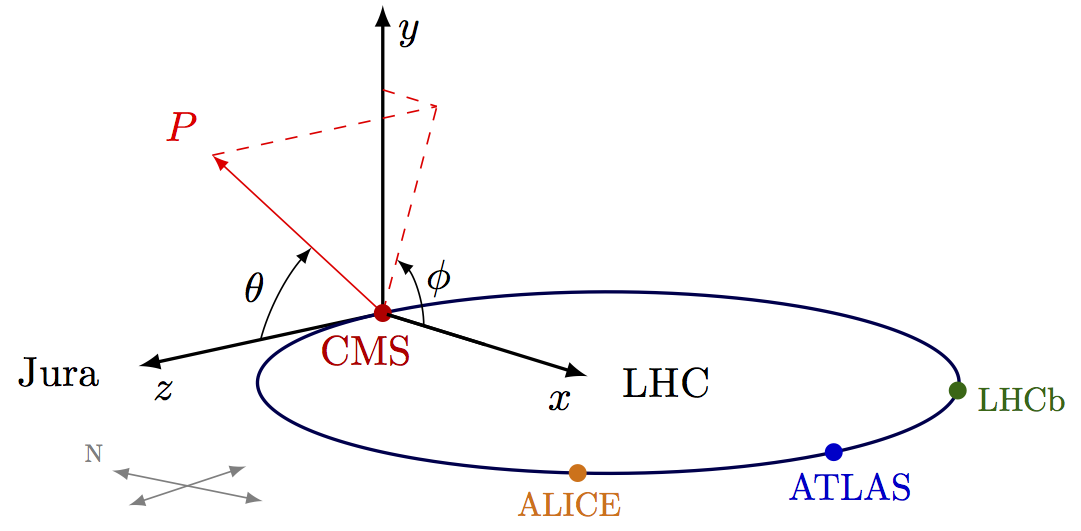
\includegraphics[width=0.8\textwidth]{Images/coordinatechart.png}
    \captionof{figure}{Coordinate system employed by the CMS experiment (retrieved from~\parencite{cmsplots}).}\label{fig_coordinates}
\end{center}

Throughout this work, phenomenological studies and comparisons are primarily developed in the context of CMS, although several results from ATLAS are also referenced, given the close alignment in sensitivity and scope. Measurements performed at CMS adopt a right-handed coordinate system with its origin at the nominal collision point. The $z$-axis is defined along the beam direction, the $x$-axis points radially inward toward the center of the LHC ring, and the $y$-axis points vertically upward. The azimuthal angle $\phi$ is measured in the transverse ($xy$) plane from the $x$-axis, while the polar angle $\theta$ is measured from the $z$-axis, as shown in Fig.~\ref{fig_coordinates}. Moreover, for kinematic analysis at hadron colliders, the Cartesian coordinate system is often reparameterized into quantities that are more physically meaningful and experimentally convenient as shown in Fig.~\ref{fig_cms_coor}:

\begin{description}
	\item[Pseudo-rapidity] $(\eta)$ Instead of using the polar angle, CMS measurements involve the pseudo-rapidity, defined by
	$$
	\eta=-\ln \left(\tan \frac{\theta}{2}\right)
	$$
	The main advantage of using the pseudo-rapidity is that distributions over it tend to be closer to a uniform distribution than those over the polar angle, see Fig.~\ref{fig_cms_coor}. Furthermore, the difference in pseudo-rapidity is invariant under Lorentz boosts along the beam direction~\parencite{book:1123430}.
	
	\item[Transverse Momentum] ($p_T$) Refers to the component of momentum which is perpendicular to the beam line. It is usually preferred over full momentum because momentum along the beamline may just be left over from the beam particles, while the transverse momentum is always associated with whatever physics happened at the vertex, see Fig.~\ref{fig_cms_coor}.
	
	\item[Azimuthal Angle] ($\phi$) Measures the angle in the transverse plane relative to the $x$-axis, providing the directional component perpendicular to the beam line.
\end{description}

\begin{center}
  		% CMS detector - left perspective
		\tdplotsetmaincoords{75}{50} % to reset previous setting
		\begin{tikzpicture}[scale=2.6,tdplot_main_coords,rotate around x=90]
			
			% VARIABLES
			\def\rvec{\L/2/cos(\thetavec)}
			\def\thetavec{18}
			\def\phivec{60}
			\def\L{3.3}    % detector length
			\def\R{0.75}   % detector cylinder radius
			\def\l{4.3}    % beam pipe length
			\def\r{0.04}   % beam pipe radius
			\def\rt{0.042} % beam pipe radius + line thickness
			\def\xmax{1}   % maximum x axis
			\def\ymax{1}   % maximum y axis
			\def\zmin{-\l/2-0.2} % minimum z axis
			\def\zmax{\l/2+0.3}  % maximum z axis
			\def\w{0.3}
			\coordinate (O) at (0,0,0);
			\coordinate (Z) at (0,0,\L/2);
			\tdplotsetcoord{O'}{0.022}{\thetavec}{\phivec} % slightly shifted origin
			\tdplotsetcoord{O''}{0.018}{90}{\phivec} % slightly shifted origin
			\tdplotsetcoord{P}{\rvec}{\thetavec}{\phivec}
			
			% CYLINDER behind
			\def\ang{19} % rotate lines to simulate cylinder
			\fill[top color=red!50!black!4,bottom color=red!60!black!2,rotate around z=\ang]
			(0,\R,\L/2) --++ (0,0,-\L) arc(90:270:\R) --++ (0,0,\L) arc(270:90:\R) -- cycle;
			\fill[detector surface] % transverse plane at z=L/2
			(0,0,\L/2) --++ (0,\R,0) arc(90:270:\R) -- cycle;
			\fill[detector surface] % transverse plane at z=-L/2
			(0,0,-\L/2) --++ (0,\R,0) arc(90:270:\R) -- cycle;
			\tdplotdrawarc[detector]{(0,0,\L/2)}{\R}{0}{360}{}{}
			\tdplotdrawarc[detector,thin]{(0,0,-\L/2)}{\R}{0}{360}{}{}
			%\draw[detector,canvas is yx plane at z=-\L/2] (0,0,0) circle(\R);
			\draw[detector,thin, dashed] % transverse plane at z=0
			(90-\ang:\R) arc (90-\ang:270:\R);
			\draw[detector] (0,0,-\L/2)++(90:\R) --++ (0,0,\L); % top horizontal
			\draw[detector] (0,0,-\L/2)++(-90:\R) --++ (0,0,\L); % bottom horizontal
			
			% BEAM PIPE
			\tdplotdrawarc[beam pipe]{(0,0,\l/2)}{\r}{0}{360}{}{}
			%\tdplotdrawarc[beam pipe]{(0,0,-\l/2)}{\r}{\ang-90}{90}{}{}
			%\draw[beam pipe] % cylindric beam pipe
			%  (0,\r,-\l/2) --++ (0,0,\l) arc(90:-90:\r)
			%  --++ (0,0,-\l) arc(-90:90:\r);
			\draw[beam pipe] % beam pipe, thinner in middle
			(0,\r,-\l/2) -- (0,\r,-0.2*\l) -- (90:0.5*\r)
			-- (0,\r,0.2*\l) -- (0,\r,0.5*\l) arc(90:-90:\r)
			-- (0,-\r,0.2*\l) -- (-90:0.5*\r) --
			(0,-\r,-0.2*\l) -- (0,-\r,-\l/2) arc(-90:90:\r);
			\draw[beam pipe] (0,0,\l/2) circle(\r);
			
			% AXES
			%\draw[thick,->] (0,0,0) -- (0,0,1) node[below right]{$z$}; % short
			\draw[axis,-] (0,0,\zmin) -- (0,0,0); % long
			\fill[CMScol] (O) circle(0.5pt) node[right=1,below=1] {IP};
			\draw[axis] (0,0,0.020) -- (0,0,\zmax) node[right=3,above=0.1]{$z$}; % long
			\draw[axis] (0,0.019,0) -- (0,\ymax,0) node[below left]{$y$};
			\draw[axis] (0.022,0,0) -- (\xmax,0,0) node[below=1,right=-2]{$x$};
			
			% LABELS
			\node[mydarkred,above] at (0,\ymax,0) {$\eta=0$};
			\node[mydarkred,above=0.6, left] at (0,\R,0.3*\L) {$\eta>0$};
			\node[mydarkred,above=0.7, right] at (0,\R,-0.2*\L) {$\eta<0$};
			\node[mydarkred,below=1,left] at (0,0,\zmax) {$\eta=\infty$};
			\node[mydarkred,above=1,right] at (0,0,\zmin) {$\eta=-\infty$};
			
			% VECTORS
			%\fill[radius=0.4,red] (P) circle;
			\draw[dashed,myred] (P)  -- (Pxy);
			\draw[dashed,myred] (Py) -- (Pxy);
			\draw[dashed,myred] (P) -- (Pz);
			
			
			\draw[->,miverde,line cap=round,draw opacity=0.9] (O') -- (P) node[anchor=-30] {\contour{white}{$\va*{p}$}};
			\draw[->,miverde,line cap=round] (O') -- (P) node[anchor=-30] {$\va*{p}$};
			
			\draw[->,azulF,line cap=round,draw opacity=0.9] (O') -- (Pxy) node[right, anchor=-100] {\contour{white}{$\va*{p}_T$}};
			% \draw[->,azulF,line cap=round] (O') -- (Pxy) node[right , anchor=-100] {$\va*{p}_T$};
			
			
			% CYLINDER front
			\draw[beam pipe,fill=none] (0,\r,-\l/2) arc(90:-90:\r);
			\fill[detector surface] % transverse plane at z=L/2
			(0,\rt,\L/2) --++ (0,\R-\rt,0) arc(90:-90:\R) --++ (0,\R-\rt,0) arc(-90:90:\rt);
			\fill[detector surface] % transverse plane at z=-L/2
			(0,\rt,-\L/2) --++ (0,\R-\rt,0) arc(90:-90:\R) --++ (0,\R-\rt,0) arc(-90:90:\rt);
			\tdplotdrawarc[detector]{(0,0,\L/2)}{\R}{-90}{90}{}{} % transverse plane at z=L/2
			\tdplotdrawarc[detector]{(0,0,-\L/2)}{\R}{-90}{90}{}{} % transverse plane at z=-L/2
			\draw[beam pipe,fill=none] (0,\r,\l/2) arc(90:-90:\r);
			\draw[detector,very thin, dashed] % transverse plane at z=0
			(90-\ang:\R) arc (90-\ang:-90:\R);
			
			% ANGLES
			\tdplotdrawarc[thick,red!57!black!3] % contour
			{(O)}{0.2}{4}{0.7*\phivec}{}{}

			% white to contour
			\tdplotdrawarc[draw=azulF, line width=0.6pt, draw opacity=0.9]{(O)}{0.2}{0}{\phivec}{above=2,right=0.75,anchor=-30,text=black}{\contour{white}{$\phi$}}
			\tdplotdrawarc[->, azulF]{(O)}{0.2}{0}{\phivec}{above=2,right=0.75,anchor=-30}{$\phi$}


			\tdplotdrawarc[->,rotate around z=\phivec-90,rotate around y=-90]
			{(O)}{0.88}{0}{\thetavec}{anchor=mid east}{$\theta$}
			\tdplotdrawarc[thick,red!58!black!4,rotate around z=\phivec-90,rotate around y=-90] % contour
			{(O)}{0.3}{88}{0.5*(90+\thetavec)}{}{}
			\tdplotdrawarc[-{>[flex'=1]},rotate around z=\phivec-90,rotate around y=-90,line cap=round]
			{(O)}{0.3}{90}{\thetavec}{above=4.5,right=0.5,anchor=mid east}{$\eta$}
			\draw[mydarkred] (0,0,\L/2) --++ (\R,0,0);
			\tdplotdrawarc[thick,red!60!black!6] % contour
			{(Z)}{0.2}{4}{0.7*\phivec}{}{}
			\tdplotdrawarc[draw=none,opacity=0.8]{(Z)}{0.2}{0}{\phivec}{above=2,right=0.7,anchor=-30}{\contour{red!60!black!6}{$\phi$}}
			\tdplotdrawarc[->]{(Z)}{0.2}{0}{\phivec}{above=2,right=0.7,anchor=-30}{$\phi$}
			
			% COMPASS - CMS-ATLAS axis has a ~12° declination (http://googlecompass.com)
			\begin{scope}[shift={(1.1*\R,-\R,0.2*\L)},rotate around y=12]
				\draw[<->,black!50] (-\w,0,0) -- (\w,0,0);
				\draw[<->,black!50] (0,0,-\w) -- (0,0,\w);
				\node[left,black!50,scale=0.6] at (-\w,0,0) {N};
				\node[below=3,left=-2,green!20!black!50,scale=0.6] at (0,0,\w) {Jura};
				%\node[below=1,right,black!50,scale=0.6,align=center] at (\w,0,0) {center of\\the LHC};
				%\node[below=1,right,blue!30!black!50,scale=0.6] at (\w,0,0) {ATLAS};
			\end{scope}
			\draw[->,thick,orange!30!black] (1.4*\w,-\R,-0.1*\L) --++ (2*\w,0,0)
			node[right,scale=0.8,align=center] {center of\\[-1pt]the LHC};
			
		\end{tikzpicture}
  \captionof{figure}{Detailed reparametrization of the coordinate system employed by the CMS experiment (retrieved from~\parencite{cmsplots})}\label{fig_cms_coor}
\end{center}

Together, the triplet $(p_T, \phi, \eta)$ forms a natural coordinate system that fully describes a particle's three-momentum vector at a hadron collider. The full four-momentum $(E, p_x, p_y, p_z)$ can be reconstructed from these quantities, typically supplemented by either the particle's mass hypothesis (for identified particles like electrons or muons) or the energy deposited in the calorimeters (for neutral objects like photons or jets). This $(p_T, \phi, \eta)$ system serves as the fundamental framework for defining physical objects, calculating event variables, and performing analyses at the LHC, providing both experimental convenience and physical insight into the collision dynamics.

A key challenge is isolating the primary hard interaction from the additional concurrent pile-up interactions. This is accomplished by reconstructing distinct interaction vertices along the beam direction and associating charged particles to their point of origin. The ultimate aim of the reconstruction chain is to identify all stable particles produced in the collision and measure their four-momenta, thereby enabling the identification of the underlying fundamental process.

\begin{center}
    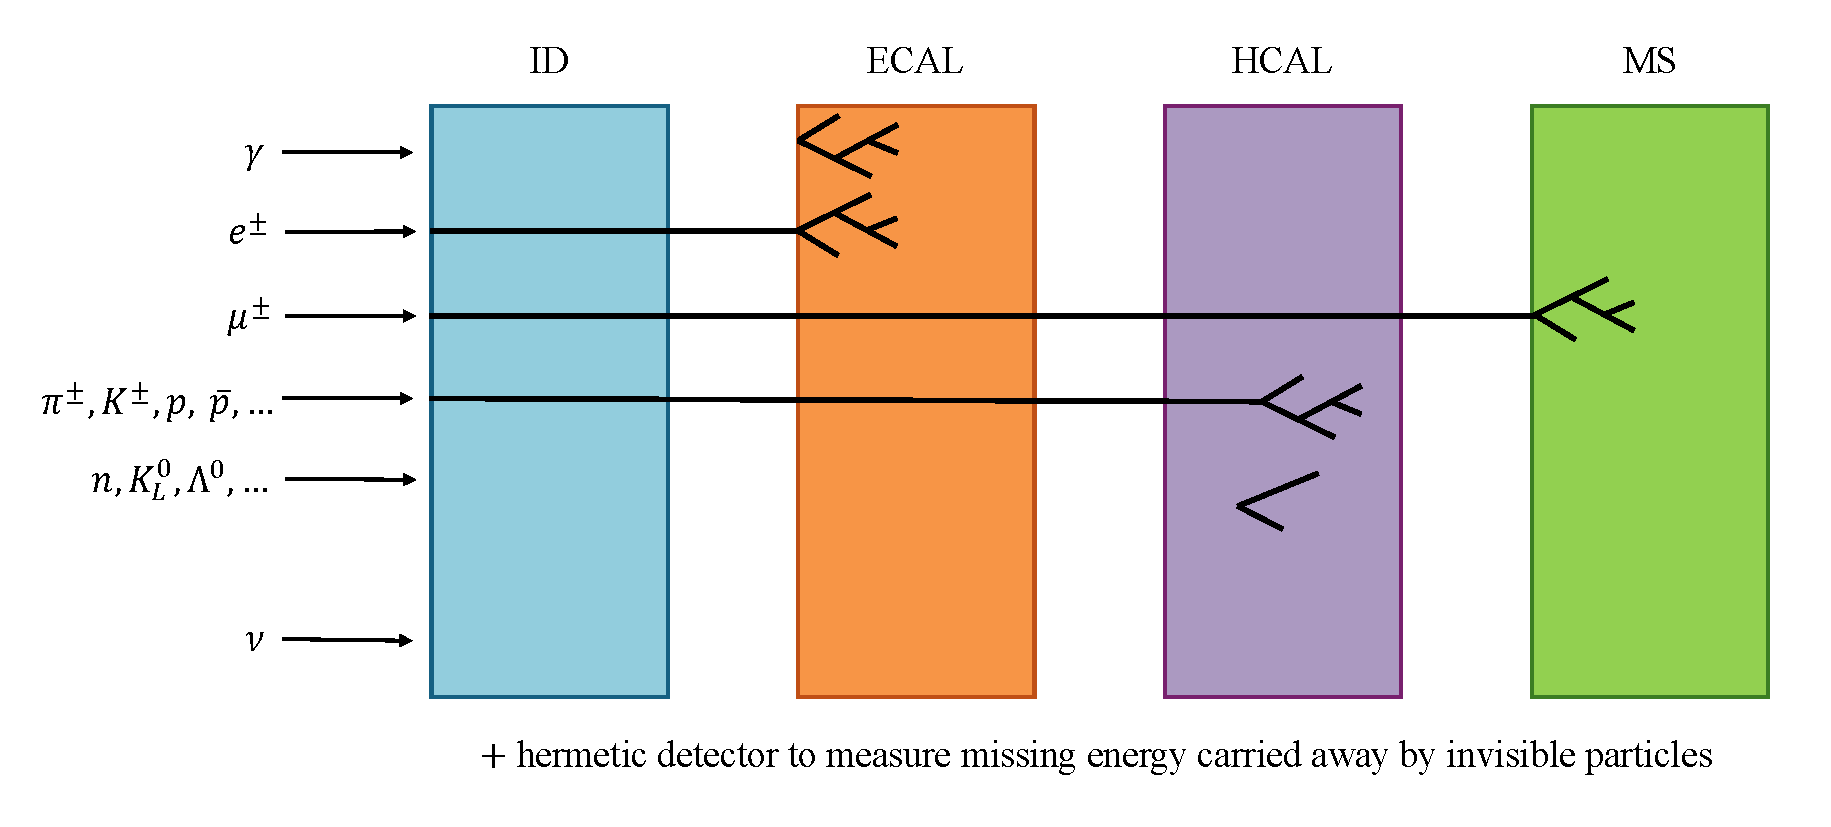
\includegraphics[width=\textwidth]{Images/Layers.pdf}
    \captionof{figure}{Illustration of high-energy particles being identified by consecutive types of subdetectors in a typical collider experiment. The curvature of the tracks in the magnetic field is not shown for simplicity. Representation of which particles and kinds of detectors are used in a multipurpose detector such as CMS or ATLAS.}\label{fig_layers}
\end{center}

However, the reconstruction is complicated by several factors. The initial state of the colliding protons is not fully known, as they are composite particles made up of quarks and gluons (collectively referred to as partons). The fraction of the proton's momentum carried by each parton is described by parton distribution functions (PDFs), which are determined experimentally. Consequently, the total momentum along the beam axis ($z$) is not balanced on an event-by-event basis. Furthermore, not all particles are stable enough to reach the detector; some decay before being detected, and only their decay products are observed. The design of a collider experiment, illustrated in Fig.~\ref{fig_layers}, is optimized for the identification and energy measurement of the particles produced in high-energy collisions.

Finally, some hypothetical particles, such as those comprising dark matter, along with known neutrinos, interact very weakly with matter and escape direct detection. Therefore, a hermetic detector design is crucial to infer their presence by accurately measuring the imbalance of energy and momentum in the transverse plane, referred to as missing transverse momentum.

\begin{center}
    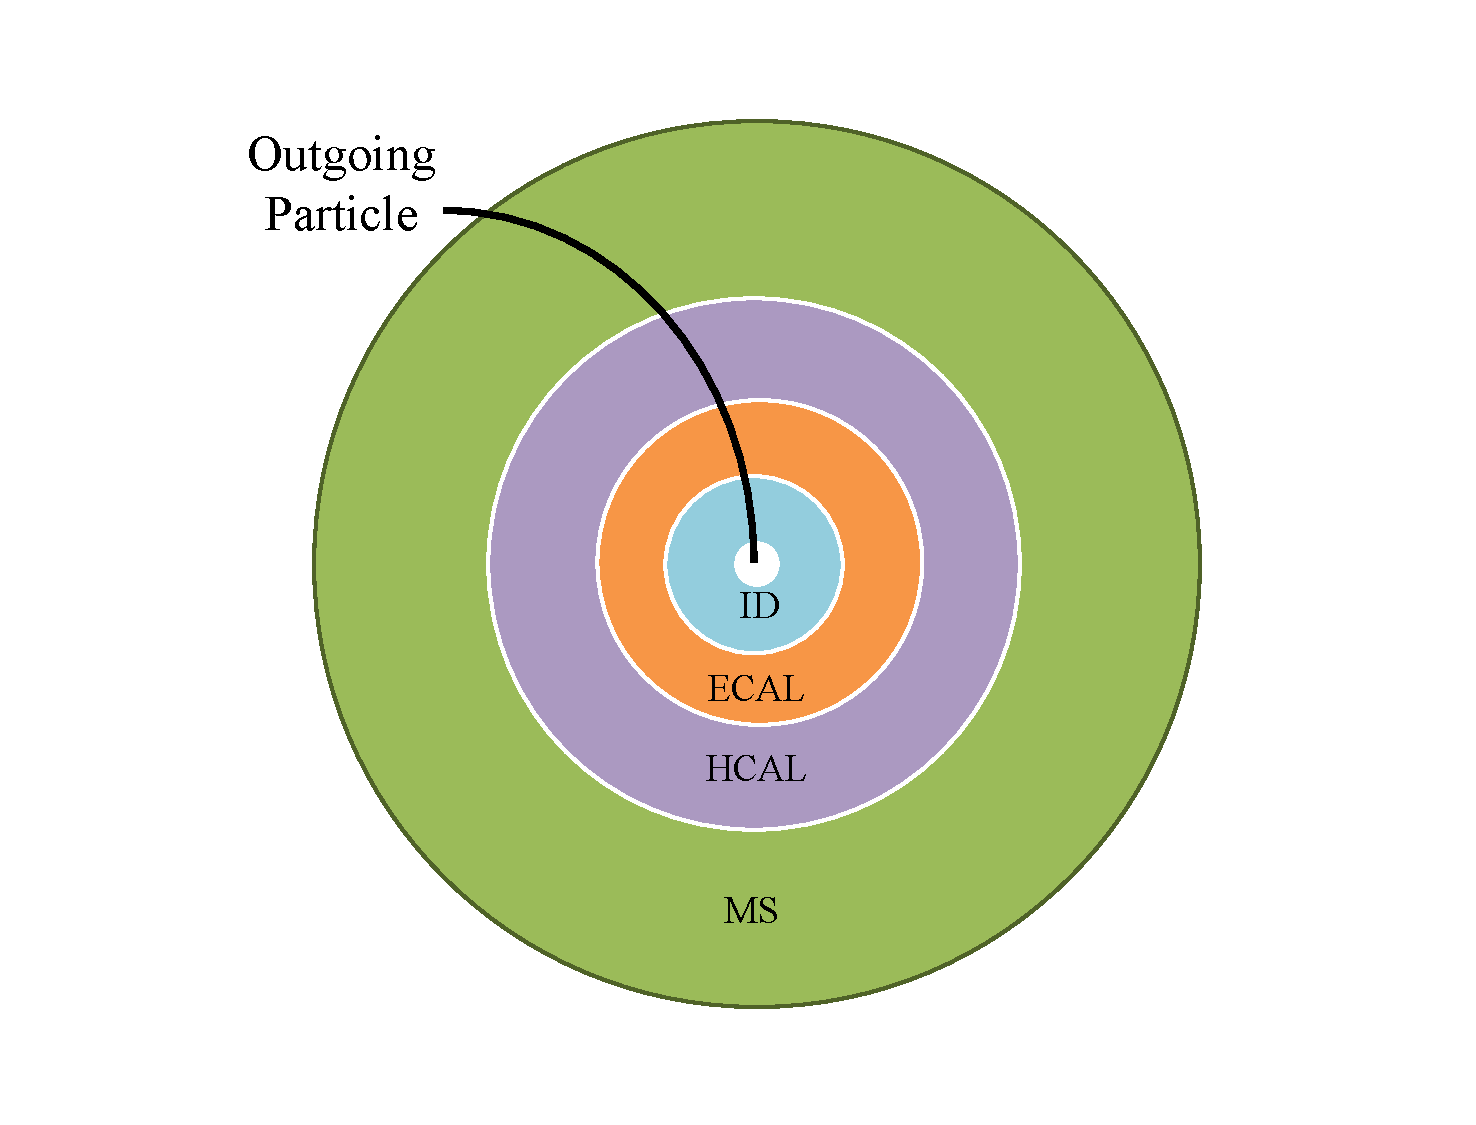
\includegraphics[width=0.85\textwidth]{Images/transversal_detector.pdf}
    \captionof{figure}{Schematic representation of a transverse section of a generic multipurpose detector. The inner detector (ID) is used to measure the trajectories of charged particles, the electromagnetic calorimeter (ECAL) measures the energy of photons and electrons, the hadronic calorimeter (HCAL) measures the energy of hadrons, and the muon system (MS) identifies and measures muons. The missing transverse momentum (MET) is inferred from the momentum imbalance in the transverse plane.}\label{fig_detector}
\end{center}

In this way, a typical collider experiment comprises several main detector subsystems that are used jointly to detect and measure the properties of particles produced in the collision. A \textit{schematic representation} of such a generic multipurpose detector is shown in Fig.~\ref{fig_detector}. The detector features an "onion-like" design of several concentric layers, each optimized to identify different types of particles and measure their properties.

The innermost subsystem, the inner detector (ID) or tracker, is immersed in a strong axial magnetic field (typically 1–4 T). It is designed to reconstruct the trajectories of charged particles, which are bent by the magnetic field. The direction and curvature of these trajectories, called \textbf{tracks}, yield the particle's momentum vector and electric charge. The most common long-lived charged particles from the SM are leptons (electrons $e$ and muons $\mu$) and hadrons (pions $\pi$, kaons $K$, and protons $p$). In some detectors, the ID is complemented by a Cherenkov light detector to measure particle velocity. Combined with the momentum measurement, this velocity helps determine the particle mass, allowing for differentiation between pions, kaons, and protons.

After the tracker, particles enter the electromagnetic calorimeter (ECAL), which is designed to fully absorb photons, electrons, and positrons. These particles deposit all their energy in the ECAL by initiating an electromagnetic shower via bremsstrahlung and $e^{+}e^{-}$ pair production. Electrons are identified as charged tracks that point to a compact, high-energy deposit in the ECAL.

The hadronic calorimeter (HCAL) surrounds the ECAL. Its purpose is to absorb hadrons (e.g., neutrons, protons, pions, kaons) and measure their energy through hadronic interactions. High-energy quarks and gluons do not appear as individual particles but instead \textbf{hadronize} into collimated sprays of hadrons known as \textbf{jets}, see Sec.~\ref{sec:jets}. A jet's energy is measured by combining the energy deposited in the ECAL and HCAL with the momenta of charged tracks associated with it. This approach, known as particle flow (PF) reconstruction, which combines information from all detector subsystems to identify each individual particle, provides a more accurate measurement.


Muons are unique as they are the only charged particles (apart from neutrinos) that can penetrate the entire calorimeter system, losing only a small amount of energy via ionization. Therefore, a dedicated muon system (MS) is built outside the calorimeters. Muons are identified as tracks in the ID that are matched to tracks in the MS. The MS, often within its own magnetic field, provides a standalone momentum measurement, which is combined with the ID measurement for high precision.

Since the detector is nearly hermetic (covering almost the full solid angle), momentum conservation in the plane transverse to the beam line ($x$-$y$ plane) is a powerful tool. The vector sum of the momenta in the transverse plane ($\vec{p}_T$) of all detected particles should be zero. Any significant imbalance indicates the presence of undetected, neutral particles that did not interact with the detector, such as neutrinos or hypothetical new particles. This imbalance is called missing transverse momentum (MET) and is formally defined as:
$$
\vec{p}_T^{\text{miss}} \equiv -\sum_i \vec{p}_{T,i}
$$
where the sum runs over all reconstructed particles (e.g., leptons, photons, jets) or calorimeter deposits in the event.

This detector design, optimized for identifying and measuring Standard Model particles, also makes it a powerful instrument for searching for new physics beyond the SM through unusual signatures or an excess of events with large MET.

\subsection{Collision Parameters}\label{sec:cross_sec_lumi}

A aim of particle physics experiments is to quantify how frequently different processes occur and to characterize the properties of the particles involved. These quantities are expressed in terms of \textbf{cross-sections}, normalized to the \textbf{luminosity} delivered by the accelerator.


The cross-section ($\sigma$) quantifies the probability for a specific process to occur. Formally, it represents the effective area of a target particle presented to an incoming beam particle for an interaction to happen. It has units of area, typically barn (b), where $1\,\text{b} = 10^{-28}\,\text{m}^2$.

In the context of proton-proton ($pp$) collisions at the LHC, the concept is generalized. Since both colliding particles are composite, the cross-section for a specific process is calculated by considering the interactions between their constituent partons (quarks and gluons). The total cross-section for a process $pp \to X$ is given by the convolution of the parton distribution functions (PDFs) and the partonic cross-section $\hat{\sigma}_{ij \to X}$:
\begin{equation}
\sigma(pp \to X) = \sum_{i,j} \int_0^1 dx_1 dx_2\, f_i(x_1, \mu_F^2) f_j(x_2, \mu_F^2)\, \hat{\sigma}_{ij \to X}(\hat{s}, \mu_F^2, \mu_R^2),
\label{eq:cross_section}
\end{equation}
where:
\begin{itemize}
    \item The sum runs over all possible parton types $i, j$ (e.g., $u, d, g$) in the two protons.
    \item $f_i(x, \mu_F^2)$ is the PDF, representing the probability density to find a parton of type $i$ carrying a fraction $x$ of the proton's momentum at a factorization scale $\mu_F$.
		\item $\hat{s} = x_1 x_2 s$ is the square of the center-of-mass energy for the colliding partons, with $s$ being the square of the $pp$ center-of-mass energy (e.g., 13.6 TeV).
    \item $\mu_R$ is the renormalization scale.
    \item $\hat{\sigma}_{ij \to X}$ is the partonic cross-section for the hard scattering process $ij \to X$.
\end{itemize}
Then, in one hand, the cross-section $\sigma$ is a theoretical quantity that encapsulates the fundamental physics of the interaction, independent of the accelerator's performance. On the other hand, the \textbf{luminosity} ($\mathcal{L}$) is a property of the particle accelerator and beams. It measures the density of particles in the colliding beams and thus the rate at which interactions can occur. The instantaneous luminosity is defined by:
\begin{equation}
\mathcal{L} = \frac{f n_1 n_2}{4\pi \sigma_x \sigma_y},
\end{equation}
where $f$ is the revolution frequency of the bunches, $n_1$ and $n_2$ are the numbers of particles in each bunch, and $\sigma_x$ and $\sigma_y$ are the transverse dimensions of the beams at the interaction point. The integrated luminosity is the integral of the instantaneous luminosity over time:
\begin{equation}
L = \int \mathcal{L}\, dt.
\end{equation}
The primary unit of integrated luminosity is the inverse barn ($\text{b}^{-1}$), commonly $\text{fb}^{-1}$.

The expected number of events ($N$) for a given process in a collider experiment connects the cross-section and integrated luminosity through the relation
\begin{equation}
N = \sigma \cdot L \cdot \epsilon.
\label{eq:N_sigma_L}
\end{equation}
Here, $\epsilon$ is the product efficiency~$\times$~acceptance of the detector for the process in question. It estimates the fraction of produced events that are actually detected and reconstructed, accounting for detector geometry, resolution, and analysis selection criteria.

On one side, if a process is known, we can measure the number of events $N$, know the integrated luminosity $L$ from accelerator measurements, and calculate the efficiency $\epsilon$ from simulation. Equation~\ref{eq:N_sigma_L} is then solved for $\sigma$ to provide a measurement of the production rate. On the other side, if we are searching for a new process not predicted by the Standard Model, we calculate the expected background $N_\text{bkg}$ from known SM processes. We then observe a number of events $N_\text{obs}$. Any significant excess, $N_\text{obs} - N_\text{bkg}$, can be interpreted as a potential signal, and Equation~\ref{eq:N_sigma_L} can be used to set an upper limit on the cross-section $\sigma_\text{BSM}$ of the hypothetical new process.

